\section{Kirurgisk behandling}

Knæet Articulatio genus, er er synovialt, sammensat led med en bevægelses grad fra (0-135\deg) flektion til (0-5\deg) ekstension. Knæledet er legemets største led, der med er det også udsat for større mekaniske påvirkninger end noget andet led i kroppen, hvilket gør at knæleddet hyppigere end noget andet led er sæde for patologiske forandringer. Knælettet er sammensat af 3 dele; femuralis, tibia og patella, disse er alle i slidfladerne beklædt med et tykt lag hyalin brusk, op til 7 mm på femur. Der sammen meniskerne, som er fibrøse brusk stykker som fordeler trykket på en større overflade, med til at mindske friktionen i leddet. [Bevægeapperatets anatomi]
//
Anatomisk billede af knæleddet, med flektions grader og enkelte sener. 
\subsection{Knæartrose}

Knæartrose også kaldet slidgigt i knæene, har mange årsager. Hvor af nogle er overvægt, arv, traume eller tungt arbejde. Arterose er karakteriseret ved ødelæggelse af ledbrusken med dertil hørende reaktioner i de tillæggende knogler og slimhinder. Symptomerne på knæartrose er smerte, funktionstab og fejlstilling, hvilket besværliggøre hverdagen. 
Ved knæartrose er sidste behandlings skridt kirurgi, afhængig af graden af traumet er forskellige kirurgiske indgreb en mulighed. [Nationale retningslinjer] 

\subsection{Osteotomi}
Osteotomi er en gennemskæring af knoglen der har tilformål at ændre knæets mekaniske akse, hvilket vil ændre belastningen af de degenererede områder. Hvilket ofte skyldes fejlstilling, Osteotomi vil være mindre invasiv end TKA og anbefales af sundhedstyrelsen til behandling af mildere former for artrose med fejlstilling hos yngre og aktive patienter. Behandlingen ses som en temporær behandling der kan udskyde behovet for TKA, ifølge et Kohordestudie kan der forventes en smertelindring os 80\% af patienterne der får udført osteotomi. (79)(80) I følge [Nationale retningslinjer] må det forventes at 30-50\% af patienterne der får foretatget en osteotomi også vil få behov for en alloplastik operation. [Nationale retningslinjer]  

\subsection{Alloplastik}
Operativt indgreb der har til formål helt eller delvist at udskifte knæleddet, med specielt designet metal og plast komponenter som varig erstatning for bruskfladerne i knæet. Operationen opdelles i totalknæalloplastik (TKA) og unikompartmentel knæalloplastik (UKA), hvilket hhv. er helt eller delvis udskiftning af knæleddet og afhænder af den specifikke diagnose. Der kan ved traume tilfælde eller svære beskadigelser af de anatomiske strukturer omkring knæet forekomme specialiserede udgaver af TKA.

\begin{figure}[H] 
\begin{center}
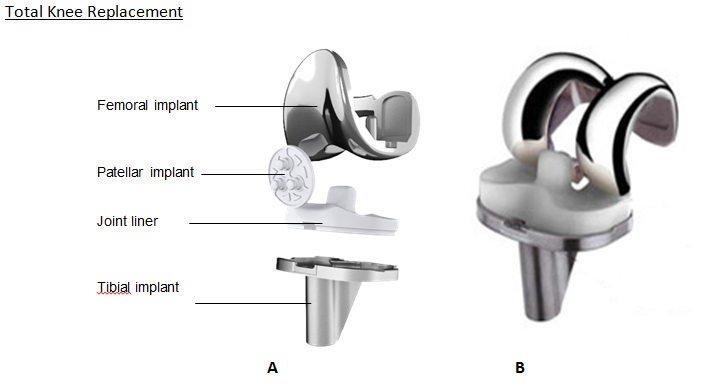
\includegraphics[width=0.7\textwidth]{figures/tka_implant}
\end{center}
\caption{Komponenterne til en total knæalloplastik, består af et femural og tibia implantat ofte bestående af en titaniumlegering. Mens patella og tibia indsatsent er lavet af polyethylen, hvilket er med til at mindske friktionen og efterligne knæledes naturlige bevægelse.\cite{1}} 
\label{fig:tka_implant} 
\end{figure}

Under selve operationen ligger patienten supineret på operationsbordet med knæet i en flekteret position, et longitudinelt snit ligges over midten af patella. Patella og senerne eleveres og blotter knæleddet, hvilket giver kirurgen adgang til bruskfladerne på femur og tibia. Herefter fjerner kirurgen det ødelagte brusk, vedhjælp af en guide blok der skruges ind i femur og sikre præcis fjernelse at den ønskede mængde væv. Dette gentages på tibia, hvorved der skabes plads til implantaterne. Midlertidige implantater indsættet for at sikre bevægelses friheden er bevaret og testes ved ekstension af knæet for at sikre at den rigtige mænge brusk og knogle materiale er fjernet. Når kirurgen er tilfreds med resultatet bordes der guide huller i hhv. femur, tibia og patella til fastemontering af de permanente implantater. Fastmontering sker ved at dække implantatet og montering stedet i bencement der limer proteserne fast til den eksisterende knogle struktur. Her efter sikres endnu engang at bevægelsesgraden er bibeholdt, førend indsnittet lukkes og operationen er fuldendt. En TKA operation vare typisk mindre en én time, hvor efter patienten kan støtte på benet den følgende dag. Efter operationen følger et rehabiliteringsforløb for at støtte og styrke muskulaturen omkring knæet. [2]

I følge sundhedsstyrelsens anbefalinger har: "Knæalloplastik har god effekt på smerte, funktion og livskva- litet som behandling af knæartrose" mens "Svær overvægt øger risikoen for komplikationer". Holdbarheden af knæ implantaterne vurderes ud fra antallet af implantater der er blevet udskiftet efter 10 år, hvor det findes at 90 til 95\% af implantaterne ikke er revideret. Dog skal nævnes at det ikke er muligt at sige noget om holdbarheden af den enkelte protese, da flertallet af patienter dør med en velfungerende protese. [Nationale retningslinjer]

(1) http://www.robodoc.com/patient_about_faqs.html

(2) https://www.youtube.com/watch?v=tKji04oFGdU

(79) Dahl AW, Toksvig-Larsen S, Roos EM. A 2-year prospective study of patient- relevant outcomes in patients operated on for knee osteoarthritis with tibial osteot- omy. BMC Musculoskeletal Disorders 2005;6(1):18.
(80) Hoell S, Suttmoeller J, Stoll V, Fuchs S, Gosheger G. The high tibial osteoto- my, open versus closed wedge, a comparison of methods in 108 patients. Arch Or- thop Trauma Surg 2005;125(9):638-643.